\chapter{Regeling van de bloeddruk en inspanning}\label{ch:b2:blood-pressure}

Sta snel op nadat je hebt gelegen en een seconde lang zakt een halve liter
\omterm{def:b2:blood-circulation:blood}{bloed} weg in de \omterm{def:b2:blood-circulation:vessels}{aders} van je benen; het \omterm{def:b2:heart:anatomy}{hart}, dat minder ontvangt, pompt
minder, de druk ter hoogte van het hoofd daalt, en de hersenen --- die een
\qty{40}{cm} boven het \omterm{def:b2:heart:anatomy}{hart} liggen en geen zuurstof kunnen opslaan --- zijn een of
twee seconden verwijderd van flauwvallen. Dat gebeurt bijna nooit, omdat een
reflex binnen één slag de \omterm{def:b2:blood-circulation:vessels}{arteriolen} heeft aangespannen en het \omterm{def:b2:heart:anatomy}{hart} heeft
versneld. Ren naar een bus en de spieren hebben tien keer het \omterm{def:b2:blood-circulation:blood}{bloed} nodig dat
ze in rust hadden; ze krijgen het binnen een minuut, en de druk die het
aandrijft, wordt stabiel gehouden terwijl de weerstand van het hele lichaam
met twee derde daalt. Dit hoofdstuk gaat over die regeling: wat de druk
bepaalt, hoe hij wordt waargenomen, de snelle reflex en de trage hormonen
die hem corrigeren, en hoe het systeem door inspanning wordt gereorganiseerd
in plaats van opzijgezet.

\section{Wat de druk is}

\begin{theorem}[De vergelijking van de bloedsomloop]\label{thm:b2:blood-pressure:equation}
\index{gemiddelde arteriële druk}\index{totale perifere weerstand}
De \omterm{thm:b2:blood-pressure:equation}{gemiddelde arteriële druk} $\bar P$ is het product van wat het \omterm{def:b2:heart:anatomy}{hart} erin
stopt en wat de vaten eruit laten:
\[
\bar P - P_{\text{ven}} = Q\,R, \qquad Q = f\times V_s,
\]
waarin $Q$ het hartminuutvolume is (hartfrequentie $f$ maal \omterm{prop:b2:heart:cycle}{slagvolume}
$V_s$), $R$ de \omterm{thm:b2:blood-pressure:equation}{totale perifere weerstand} --- de \omterm{def:b2:blood-circulation:vessels}{arteriolen} van alle organen
parallel geschakeld --- en $P_{\text{ven}}$ de veneuze druk, bijna nul. In
rust geeft $\qty{5}{L/min}\times\qty{1.08}{mmHg.s/mL}$ een druk van
\qty{90}{mmHg}. Elke regeling van de druk werkt in op een van drie
grootheden: de frequentie, het \omterm{prop:b2:heart:cycle}{slagvolume} (via de vulling en de
contractiliteit van \cref{ch:b2:heart}) of de weerstand (via de straal van
de \omterm{def:b2:blood-circulation:vessels}{arteriolen}, tot de vierde macht). Omdat de organen parallel staan, is de
stroom naar elk orgaan zijn deel van de druk gedeeld door zijn eigen
weerstand: het verwijden van de \omterm{def:b2:blood-circulation:vessels}{arteriolen} van één orgaan verhoogt zijn
stroom zonder die van de andere te veranderen, op voorwaarde dat de druk
wordt vastgehouden --- en het vasthouden van de druk is waartoe de regeling
dient.
\end{theorem}
\begin{proof}
De wet van Ohm voor een vloeistof: de stroom door een weerstand is de drukval
erover gedeeld door de weerstand (Poiseuille,
\cref{ch:b2:blood-circulation}); voor parallel geschakelde weerstanden tellen
de stromen op en is $1/R = \sum 1/R_i$. De gemiddelde druk over een slag is
bij benadering de diastolische druk plus een derde van de \omterm{thm:b2:blood-circulation:windkessel}{polsdruk}:
$80 + 40/3 = \qty{93}{mmHg}$.
\end{proof}

\begin{omfigure}
\begin{tikzpicture}[every node/.style={font=\scriptsize}, >=stealth]
  \node[draw, rounded corners, fill=omThm!15, minimum width=2.4cm, minimum height=1cm, align=center] (heart) at (0,0) {hart\\$Q = f\,V_s$};
  \draw[very thick, omThm] (1.2,0) -- (2.4,0);
  \draw[very thick, omThm] (2.4,-2.4) -- (2.4,2.4);
  \foreach \y/\org/\r in {2.0/{hersenen}/{$R_1$}, 1.0/{hartspier}/{$R_2$}, 0/{darm en lever}/{$R_3$}, -1.0/{nieren}/{$R_4$}, -2.0/{spieren, huid}/{$R_5$}} {
    \draw[very thick, omThm] (2.4,\y) -- (3.6,\y);
    \draw[thick, decorate, decoration={zigzag, segment length=4pt, amplitude=2pt}] (3.6,\y) -- (5.0,\y);
    \node[above] at (4.3,\y+0.05) {\org};
    \node[below] at (4.3,\y-0.05) {\r};
    \draw[very thick, omDef] (5.0,\y) -- (6.2,\y);
  }
  \draw[very thick, omDef] (6.2,-2.4) -- (6.2,2.4);
  \draw[very thick, omDef] (6.2,0) -- (7.4,0) |- (0,-3.2) -- (0,-0.5);
  \node[omThm, above] at (1.8,0.05) {$\bar P$};
  \node[omDef, below] at (3.7,-3.2) {aders, $P_{\text{ven}} \approx 0$};
  \node[anchor=west, align=left] at (7.8,1.5) {organen parallel:\\$1/R = \sum 1/R_i$\\stroom naar orgaan $i$: $\bar P/R_i$};
\end{tikzpicture}

{\small De bloedsomloop als een schakeling: één pomp, één druk, en de
arteriolaire weerstanden van de organen parallel. Elk orgaan neemt
$\bar P/R_i$; de regeling houdt $\bar P$ vast terwijl de $R_i$ aan de vraag
worden aangepast.}
\end{omfigure}

\begin{proposition}[Waarom de druk moet worden geregeld]\label{prop:b2:blood-pressure:why}
Te laag, en de hersenen --- bij een staande volwassene \qty{40}{cm} boven het
\omterm{def:b2:heart:anatomy}{hart}, wat \qty{31}{mmHg} hydrostatische hoogte kost --- en de hartspier zelf
worden onvoldoende doorbloed: de hersenen vallen binnen seconden uit. Te
hoog, en de vaten raken beschadigd: de slagaderwand verdikt en verstijft, de
glomeruli van de nier verlittekenen, het netvlies bloedt, en het \omterm{def:b2:heart:anatomy}{hart} zwoegt
tegen de druk in tot het faalt. De druk moet ook stabiel blijven terwijl de
vraag van de organen een orde van grootte verandert --- de darm na een
maaltijd, de spieren bij inspanning, de huid bij hitte --- en terwijl het
bloedvolume zelf verloren gaat door een bloeding of door zweten. Twee
systemen doen dit: een zenuwreflex die binnen één slag inwerkt op de
frequentie, het \omterm{prop:b2:heart:cycle}{slagvolume} en de weerstand, en hormonale systemen die over
uren en dagen inwerken op de weerstand en, vooral, via de nier op het
bloedvolume.
\end{proposition}

\begin{omfigure}
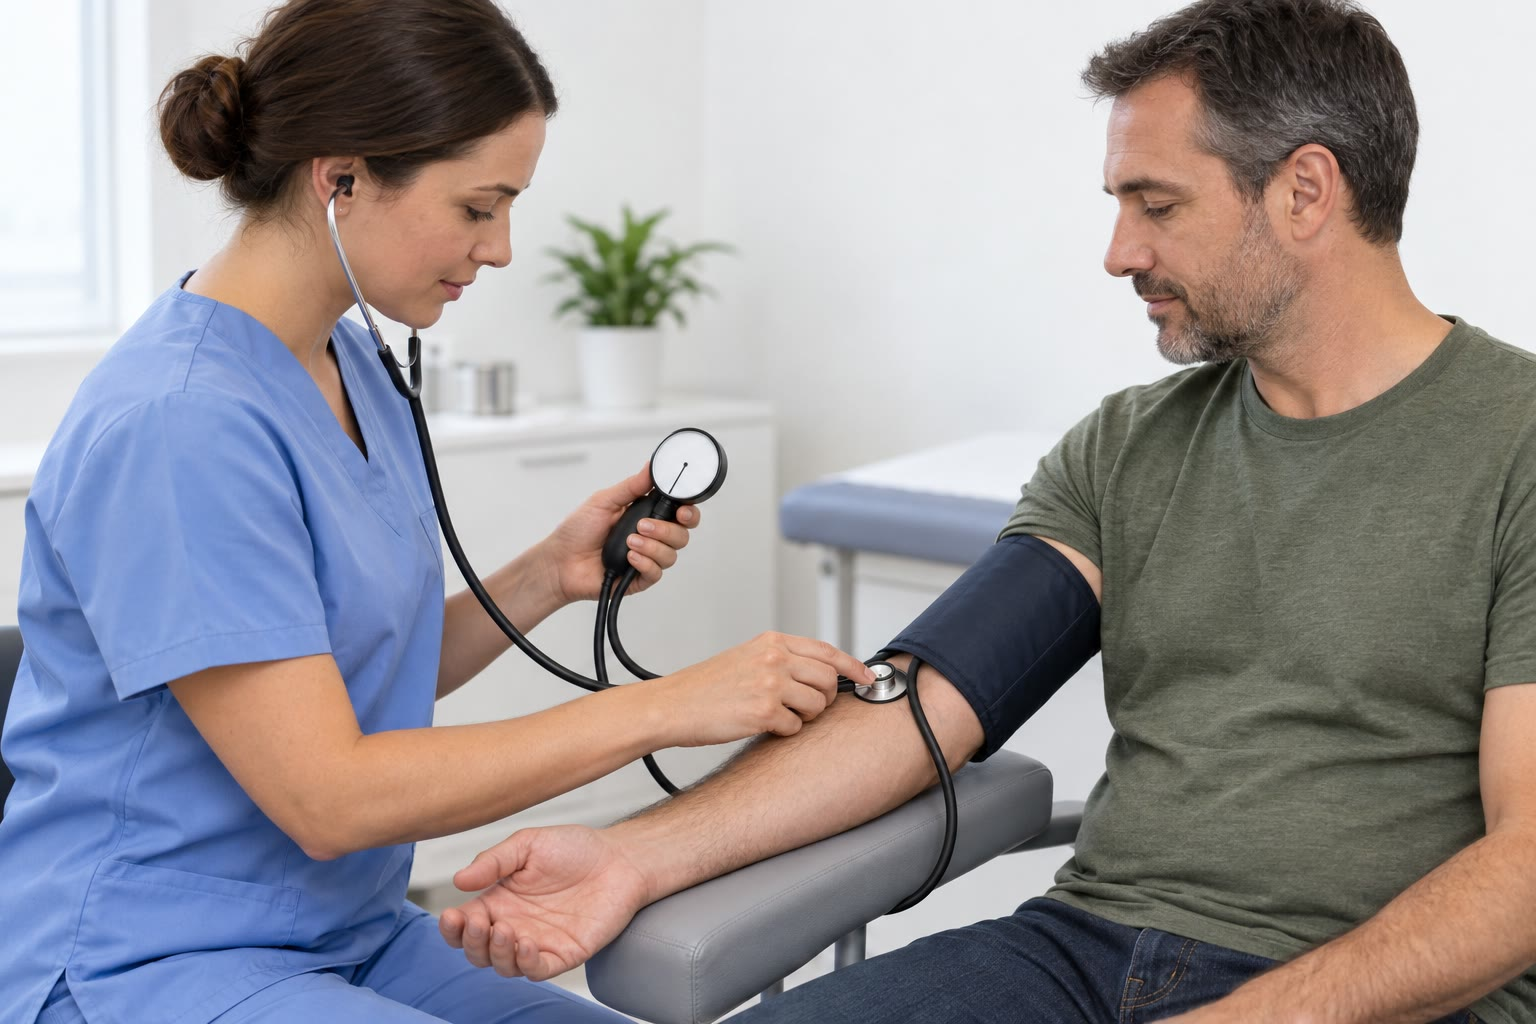
\includegraphics[width=0.6\linewidth]{images/book4/ai/b4-18-blood-pressure-cuff.jpg}

{\small Het meten van de druk. De manchet wordt opgeblazen boven de
systolische druk, zodat er geen \omterm{def:b2:blood-circulation:blood}{bloed} doorgaat; wanneer de lucht wordt
afgelaten, markeren de eerste geluiden van turbulente stroming onder de
stethoscoop de systolische druk, en hun verdwijnen, wanneer de \omterm{def:b2:blood-circulation:vessels}{slagader} de
hele cyclus open blijft, de diastolische.}
\end{omfigure}

\section{De snelle lus: de baroreflex}

\begin{definition}[De baroreflex]\label{def:b2:blood-pressure:baroreflex}
\index{baroreceptor}\index{baroreflex}\index{vasomotorisch centrum}\index{autonoom zenuwstelsel}
Rekreceptoren in de wanden van de sinus caroticus (bij de splitsing van
elke halsslagader, onder de kaak) en van de aortaboog --- de
\emph{baroreceptoren} --- vuren met een frequentie die stijgt met de druk die
ze uitrekt, en sneller bij een stijgende druk. Hun zenuwen bereiken de
\emph{cardiovasculaire centra} van het verlengde merg, die de twee takken
van de autonome uitstroom sturen: de \omterm{prop:b2:heart:control}{nervus vagus}, waarvan de acetylcholine
de sinusknoop vertraagt, en de sympathische zenuwen, waarvan de noradrenaline
de sinusknoop versnelt, het \omterm{def:b2:heart:anatomy}{ventrikel} versterkt, de \omterm{def:b2:blood-circulation:vessels}{arteriolen} vernauwt
(wat $R$ verhoogt) en de \omterm{def:b2:blood-circulation:vessels}{aders} vernauwt (wat opgeslagen \omterm{def:b2:blood-circulation:blood}{bloed} naar het \omterm{def:b2:heart:anatomy}{hart}
perst en de vulling verhoogt). Een stijging van de druk verhoogt het vuren
van de baroreceptoren, wat de \omterm{prop:b2:heart:control}{nervus vagus} prikkelt en de sympathische
uitstroom remt: de frequentie daalt, de \omterm{def:b2:blood-circulation:vessels}{arteriolen} ontspannen, de druk daalt.
Een daling doet het omgekeerde. De lus is een \emph{negatieve
terugkoppeling} met een instelwaarde bij ongeveer \qty{95}{mmHg}, een
vertraging van ongeveer een seconde, en een versterking waardoor een
verstoring tot op een vijfde van haar grootte wordt gecorrigeerd: ze is de
reden waarom je niet flauwvalt als je opstaat.
\end{definition}
\begin{proof}[Bewijsmateriaal]
Hering (1923) vond dat drukken op de sinus caroticus het \omterm{def:b2:heart:anatomy}{hart} vertraagde en
de druk verlaagde, en dat het doorsnijden van de sinuszenuw de respons ophief.
Perfusie van een geïsoleerde sinus caroticus bij ingestelde drukken, terwijl
de arteriële druk van het dier werd geregistreerd, gaf de sigmoïde curve van
de reflex: de druk van het dier daalt naarmate de sinusdruk wordt verhoogd,
steil rond \qty{100}{mmHg} en weinig buiten \qtyrange{60}{160}{mmHg}.
Honden bij wie zowel de sinus- als de aortazenuwen zijn doorgesneden,
behouden over dagen een normale gemiddelde druk, maar een wild wisselende van
minuut tot minuut --- de reflex is een buffer, niet wat het niveau op lange
termijn vastlegt.
\end{proof}

\begin{omfigure}
\begin{tikzpicture}[every node/.style={font=\scriptsize}, >=stealth]
  \node[draw, rounded corners, fill=omDef!15, align=center] (bp) at (0,0) {arteriële druk\\$\bar P$};
  \node[draw, rounded corners, fill=omDef!15, align=center] (baro) at (4.2,0) {baroreceptoren\\sinus caroticus, aortaboog\\vuurfrequentie $\uparrow$ met $\bar P$};
  \node[draw, rounded corners, fill=omProp!20, align=center] (med) at (8.6,0) {verlengde merg:\\cardiovasculaire centra};
  \node[draw, rounded corners, fill=omThm!15, align=center] (vag) at (8.6,-2.2) {vagus $\uparrow$: frequentie $\downarrow$};
  \node[draw, rounded corners, fill=omThm!15, align=center] (sym) at (4.2,-2.2) {sympathisch $\downarrow$: frequentie, contractiliteit,\\arteriolaire en veneuze tonus $\downarrow$};
  \draw[->, thick] (bp) -- (baro); \draw[->, thick] (baro) -- (med);
  \draw[->, thick] (med) -- (vag); \draw[->, thick] (med) -- (sym);
  \draw[->, thick] (sym.west) -| (bp.south) node[pos=0.75, left, align=right] {$Q\downarrow$, $R\downarrow$:\\$\bar P\downarrow$};
  \draw[->, thick] (vag.west) -- (sym.east);
  \node[anchor=north, align=center] at (4.3,-3.2) {een stijging van de druk wordt beantwoord met een daling: negatieve terugkoppeling, één seconde vertraging};
\end{tikzpicture}

{\small De \omterm{def:b2:blood-pressure:baroreflex}{baroreflex}. Een stijging van de arteriële druk verhoogt het vuren
van de \omterm{def:b2:blood-pressure:baroreflex}{baroreceptoren}, wat het verlengde merg aanzet het \omterm{def:b2:heart:anatomy}{hart} te vertragen
en de vaten te ontspannen; een daling doet het omgekeerde.}
\end{omfigure}

\begin{theorem}[Versterking van een negatieve terugkoppelingslus]\label{thm:b2:blood-pressure:gain}
\index{versterking van de terugkoppeling}
Als een verstoring de druk zonder regeling met $\Delta P_0$ zou veranderen,
en de lus op elke afwijking $\Delta P$ reageert met een correctie van
$-G\,\Delta P$ (de \emph{openlusversterking} $G$), dan is de afwijking die
overblijft nadat de lus heeft ingegrepen
\[
\Delta P = \frac{\Delta P_0}{1 + G}.
\]
De \omterm{def:b2:blood-pressure:baroreflex}{baroreflex} heeft $G \approx 4$: opstaan, wat de druk ter hoogte van het
\omterm{def:b2:heart:anatomy}{hart} met zo'n \qty{40}{mmHg} zou doen dalen, laat hem met \qty{8}{mmHg}
dalen; een bloeding die de druk zou halveren, verlaagt hem met een tiende ---
tot het verlies groter wordt dan wat nauwere vaten en een sneller \omterm{def:b2:heart:anatomy}{hart} kunnen
verbergen. De reflex heft een verstoring niet op; hij deelt haar door vijf.
En hij \emph{stelt zich opnieuw in}: urenlang op een nieuwe druk gehouden,
passen de \omterm{def:b2:blood-pressure:baroreflex}{baroreceptoren} zich aan en verdedigen ze het nieuwe niveau, en
daarom kan de reflex hypertensie niet genezen en wordt het niveau op lange
termijn elders vastgelegd.
\end{theorem}
\begin{proof}
De uiteindelijke afwijking is de verstoring plus de correctie:
$\Delta P = \Delta P_0 - G\,\Delta P$, dus $\Delta P(1 + G) =
\Delta P_0$. Met $G = 4$ is $\Delta P = \Delta P_0/5$.
\end{proof}

\begin{omfigure}
\begin{tikzpicture}
\begin{axis}[
  width=0.7\linewidth, height=5.4cm,
  axis x line=bottom, axis y line=left,
  xmin=40, xmax=180, ymin=40, ymax=160,
  xlabel={druk in de sinus caroticus (\unit{mmHg})}, ylabel={resulterende arteriële druk (\unit{mmHg})},
  xlabel style={font=\small, at={(axis description cs:0.5,-0.13)}, anchor=north},
  ylabel style={font=\small},
  tick label style={font=\small}, xtick={60,100,140}, ytick={60,100,140},
  clip=false,
]
\addplot[very thick, omDef, domain=40:180, samples=80] {100 + 50*tanh((100-x)/25)};
\addplot[thick, dashed, gray, domain=40:180, samples=2] {x};
\fill[omDef] (axis cs:100,100) circle (2pt); \draw[gray] (axis cs:101,100) -- (axis cs:124,110); \node[font=\scriptsize, anchor=west] at (axis cs:125,110) {instelwaarde};
\node[font=\scriptsize, anchor=west, align=left] at (axis cs:46,112) {helling $-G$\\bij de instelwaarde};
\end{axis}
\end{tikzpicture}

{\small De curve van de \omterm{def:b2:blood-pressure:baroreflex}{baroreflex}: de druk waarop het lichaam uitkomt
wanneer de geïsoleerde sinus op een gegeven druk wordt gehouden. De helling
bij de instelwaarde is de versterking; buiten \qtyrange{60}{160}{mmHg} is de
reflex verzadigd.}
\end{omfigure}

\section{De trage lussen: hormonen en de nier}

\begin{proposition}[Renine, angiotensine, aldosteron en het volume]\label{prop:b2:blood-pressure:raas}
\index{renine-angiotensinesysteem}\index{aldosteron}\index{antidiuretisch hormoon}\index{natriuretisch peptide}
Over uren en dagen wordt de druk bepaald door het \emph{bloedvolume}, en het
volume door de nier. Wanneer de druk of het natrium dat de nier bereikt
daalt, of de sympathische zenuwen vuren, geven cellen van de \omterm{def:b2:blood-circulation:vessels}{arteriolen} van
de nier het enzym \emph{renine} aan het \omterm{def:b2:blood-circulation:blood}{bloed} af; renine knipt een
plasma-eiwit tot \emph{angiotensine I}, dat door een enzym van de \omterm{def:b2:blood-circulation:vessels}{haarvaten}
van de long wordt omgezet in \emph{angiotensine II} --- de krachtigste
vaatvernauwer van het lichaam, die $R$ binnen minuten verhoogt, en een
hormoon dat de bijnierschors \emph{aldosteron} laat afscheiden, dat de nier
in de dagen daarna natrium, en daarmee water, laat vasthouden. Het
\emph{\omterm{prop:b2:blood-pressure:raas}{antidiuretisch hormoon}} (vasopressine) van de hypofyse, dat vrijkomt
wanneer het \omterm{def:b2:blood-circulation:blood}{bloed} geconcentreerder wordt of het volume daalt, laat de nier
rechtstreeks water vasthouden en vernauwt ook vaten. En wanneer de atria door
te veel volume worden overrekt, scheiden ze \emph{\omterm{prop:b2:blood-pressure:raas}{natriuretisch peptide}} af,
dat de nier natrium en water laat uitscheiden. De nier is dus de uiteindelijke
scheidsrechter: ze kan liters uitscheiden of vasthouden, en een druk die boven
de instelwaarde van de nier blijft, wordt over dagen gecorrigeerd door verlies
van volume --- tenzij de instelwaarde van de nier zelf is verhoogd, en dat is
wat de meeste hypertensie is. (De eigen machinerie van de nier is het
onderwerp van het deel van jaar 3.)
\end{proposition}
\begin{proof}[Bewijsmateriaal]
Goldblatt (1934) vernauwde bij een hond de \omterm{def:b2:blood-circulation:vessels}{slagader} naar één nier: het dier
werd binnen enkele dagen hypertensief en bleef dat; de onvoldoende
doorbloede nier bleek renine af te geven, en het verwijderen ervan genas het
dier. Middelen die de omzetting van angiotensine blokkeren (ACE-remmers) of
zijn receptor blokkeren, verlagen de druk van de meeste mensen met
hypertensie, en een nier die wordt getransplanteerd uit een hypertensieve
rattenstam, maakt een normale ontvanger hypertensief.
\end{proof}

\begin{omfigure}
\begin{tikzpicture}[every node/.style={font=\scriptsize}, >=stealth]
  \node[draw, rounded corners, fill=omDef!15, align=center] (fall) at (0,0) {druk of volume daalt;\\sympathische zenuwen vuren};
  \node[draw, rounded corners, fill=omProp!20, align=center] (renin) at (4.4,0) {nier geeft\\renine af};
  \node[draw, rounded corners, fill=omProp!20, align=center] (ang) at (8.6,0) {angiotensine II\\(gemaakt in bloed en long)};
  \node[draw, rounded corners, fill=omThm!15, align=center] (vc) at (8.6,-2.0) {vaatvernauwing:\\$R\uparrow$ binnen minuten};
  \node[draw, rounded corners, fill=omThm!15, align=center] (ald) at (4.4,-2.0) {aldosteron (bijnier):\\Na$^+$ en water vastgehouden\\over dagen --- volume $\uparrow$};
  \draw[->, thick] (fall) -- (renin); \draw[->, thick] (renin) -- (ang);
  \draw[->, thick] (ang) -- (vc); \draw[->, thick] (ang) -- (ald);
  \draw[->, thick] (ald.west) -| (fall.south) node[pos=0.85, left, align=right] {druk\\hersteld};
  \draw[->, thick] (vc.west) -- (ald.east);
  \node[draw, rounded corners, fill=omExo!25, align=center] (anp) at (0,-2.0) {atria overrekt:\\natriuretisch peptide,\\zout en water uitgescheiden};
  \draw[->, thick, dashed] (anp.north) -- (fall.south);
\end{tikzpicture}

{\small De trage lus. Een daling van de druk zet renine, angiotensine II en
aldosteron in gang: vernauwing binnen minuten, vasthouden van zout en water
over dagen. Te veel volume wordt beantwoord met het \omterm{prop:b2:blood-pressure:raas}{natriuretisch peptide} van
de atria.}
\end{omfigure}

\begin{example}[Een bloeding]\label{ex:b2:blood-pressure:haemorrhage}
Een donor geeft \qty{500}{mL}, een tiende van het \omterm{def:b2:blood-circulation:blood}{bloed}. Binnen seconden
vernauwt de \omterm{def:b2:blood-pressure:baroreflex}{baroreflex} de \omterm{def:b2:blood-circulation:vessels}{arteriolen} en \omterm{def:b2:blood-circulation:vessels}{aders} en versnelt hij het \omterm{def:b2:heart:anatomy}{hart}: de
druk verandert nauwelijks, de huid wordt bleek en koel (haar \omterm{def:b2:blood-circulation:vessels}{arteriolen} zijn
dicht), de pols is sneller. Binnen minuten laat de verlaagde druk in de
\omterm{def:b2:blood-circulation:vessels}{haarvaten} interstitieel vocht de vaten binnenstromen (het evenwicht van
Starling uit \cref{ch:b2:blood-circulation}), wat binnen het volgende uur de
helft van het volume herstelt; renine, angiotensine en \omterm{prop:b2:blood-pressure:raas}{antidiuretisch hormoon}
brengen de urine terug tot een straaltje, en er volgt dorst; over dagen houdt
de nier zout en water vast en is het plasmavolume terug, en over weken
vervangt het beenmerg de rode bloedcellen. Een verlies van \qty{2}{L} loopt
hier allemaal op vooruit: de reflex is verzadigd, de druk stort in, de
onvoldoende doorbloede weefsels geven lactaat af en de \omterm{def:b2:blood-circulation:vessels}{haarvaten} gaan
lekken --- shock, waaruit alleen een transfusie de patiënt terughaalt.
\end{example}

\section{Inspanning: het systeem gereorganiseerd}

\begin{proposition}[Inspanning]\label{prop:b2:blood-pressure:exercise}
\index{inspanningsfysiologie}\index{spierdoorbloeding}\index{hartminuutvolume!bij inspanning}
Bij zware inspanning stijgt het zuurstofverbruik van de skeletspieren
twintigvoudig, en hun doorbloeding van \qty{1}{L/min} tot \qty{20}{L/min}.
Er gebeuren drie dingen tegelijk. Plaatselijk ontspannen de metabolieten van
de werkende spier --- $\mathrm{CO_2}$, lactaat, adenosine, kalium, warmte,
een lage zuurstofspanning --- haar \omterm{def:b2:blood-circulation:vessels}{arteriolen} (\emph{metabole vasodilatatie})
en openen ze de \omterm{def:b2:blood-circulation:vessels}{haarvaten}, waardoor de weerstand van de spier tot een tiende
daalt. Centraal stelt een bevel van de motorische schors aan het verlengde
merg, versterkt door signalen van de eigen receptoren van de spieren, de
\omterm{def:b2:blood-pressure:baroreflex}{baroreflex} op een hogere instelwaarde in en drijft het de sympathische
uitstroom aan: frequentie naar 180, contractiliteit omhoog, de \omterm{def:b2:blood-circulation:vessels}{arteriolen} van
darm, nieren en rustende spieren vernauwd, de \omterm{def:b2:blood-circulation:vessels}{aders} samengeperst; de spierpomp
en de diepe ademhaling voeren het \omterm{def:b2:blood-circulation:blood}{bloed} sneller terug. Het resultaat is een
debiet van \qty{25}{L/min} bij een totale weerstand van een derde van de
rustwaarde, een systolische druk van \qty{150}{mmHg} en een diastolische die
niet hoger is dan in rust; vier vijfde van de stroom gaat naar de spieren,
het aandeel van de hersenen blijft in absolute zin gelijk, dat van de darm
halveert, dat van de huid stijgt om de warmte af te voeren. De reflex wordt
niet opzijgezet maar anders afgestemd: hij verdedigt een hogere druk terwijl
de vaten het lichaam weer openzetten.
\end{proposition}

\begin{omfigure}
\begin{tikzpicture}
\begin{axis}[
  ybar, bar width=9pt,
  width=0.9\linewidth, height=6cm,
  ymin=0, ymax=22, ytick={0,5,10,15,20},
  ylabel={doorbloeding (\unit{L/min})}, ylabel style={font=\small},
  symbolic x coords={hersenen, hart, darm en lever, nieren, spieren, huid, overige},
  xtick=data, x tick label style={font=\scriptsize, rotate=30, anchor=north east},
  tick label style={font=\small},
  legend style={font=\scriptsize, at={(0.03,0.97)}, anchor=north west, draw=none},
  enlarge x limits=0.12,
  clip=false,
]
\addplot[fill=omDef!50, draw=omDef] coordinates {(hersenen,0.75) (hart,0.25) (darm en lever,1.4) (nieren,1.1) (spieren,1.0) (huid,0.3) (overige,0.2)};
\addlegendentry{rust, \qty{5}{L/min}}
\addplot[fill=omThm!50, draw=omThm] coordinates {(hersenen,0.75) (hart,1.0) (darm en lever,0.6) (nieren,0.6) (spieren,20) (huid,1.6) (overige,0.45)};
\addlegendentry{zware inspanning, \qty{25}{L/min}}
\end{axis}
\end{tikzpicture}

{\small Waar het \omterm{def:b2:blood-circulation:blood}{bloed} naartoe gaat. Bij zware inspanning stijgt het debiet
vijfvoudig en wordt het herverdeeld: twintigvoudig naar de spieren, meer naar
\omterm{def:b2:heart:anatomy}{hart} en huid, minder naar darm en nieren, evenveel naar de hersenen.}
\end{omfigure}

\begin{theorem}[Zuurstoflevering en het principe van Fick]\label{thm:b2:blood-pressure:fick}
\index{principe van Fick}\index{VO2max@$\dot V_{\mathrm{O_2}\max}$}
De zuurstof die een lichaam per minuut verbruikt, is gelijk aan het
hartminuutvolume maal het verschil in zuurstofgehalte tussen arterieel en
gemengd veneus \omterm{def:b2:blood-circulation:blood}{bloed}:
\[
\dot V_{\mathrm{O_2}} = Q\,(C_a - C_v).
\]
In rust geeft dat $\qty{5}{L/min}\times(200 - 150)\,\unit{mL/L} = \qty{250}{mL/min}$;
bij maximale inspanning $\qty{25}{L/min}\times(200 - 40) =
\qty{4000}{mL/min}$, een zestienvoudige stijging uit een vijfvoudige stijging
van de stroom en een drievoudige stijging van de extractie. Deze maximale
waarde, $\dot V_{\mathrm{O_2}\max}$, is de standaardmaat voor
uithoudingsvermogen, en haar plafond is het \omterm{def:b2:heart:anatomy}{hart}: de spieren zouden nog meer
kunnen onttrekken en de longen nog meer kunnen opladen, maar het debiet kan
niet verder stijgen. Training verhoogt het \omterm{prop:b2:heart:cycle}{slagvolume} (een groter, rekbaarder
\omterm{def:b2:heart:anatomy}{ventrikel}, meer bloedvolume) en daarmee het debiet --- de rustfrequentie van
45 van de atleet is het teken van een \omterm{prop:b2:heart:cycle}{slagvolume} van \qty{110}{mL} --- en
voegt \omterm{def:b2:blood-circulation:vessels}{haarvaten} en mitochondriën aan de spier toe, zodat die meer onttrekt.
Omgekeerd is het \omterm{thm:b2:blood-pressure:fick}{principe van Fick} de manier waarop het debiet zelf bij een
patiënt wordt gemeten, uit de verbruikte zuurstof en de twee bloedmonsters.
\end{theorem}
\begin{proof}
Elke liter \omterm{def:b2:blood-circulation:blood}{bloed} die door de weefsels stroomt, laat $C_a - C_v$ milliliter
zuurstof achter, en per minuut stromen er $Q$ liter door; in de stationaire
toestand is dat wat de longen opnemen en het lichaam verbruikt. Oplossen naar
$Q$ geeft de meting.
\end{proof}

\begin{example}[Opstaan, flauwvallen en de astronaut]\label{ex:b2:blood-pressure:standing}
Bij het opstaan verschuift \qty{500}{mL} \omterm{def:b2:blood-circulation:blood}{bloed} naar de \omterm{def:b2:blood-circulation:vessels}{aders} van de benen,
dalen de veneuze terugvloed en het \omterm{prop:b2:heart:cycle}{slagvolume} met een derde, en daalt de druk
in de sinus caroticus --- de \omterm{def:b2:blood-pressure:baroreflex}{baroreflex} antwoordt binnen één slag met een
sneller \omterm{def:b2:heart:anatomy}{hart} en nauwere vaten, en de druk ter hoogte van het hoofd is binnen
tien seconden terug. Een soldaat die roerloos op een heet paradeplein staat,
verliest de spierpomp, laat \omterm{def:b2:blood-circulation:blood}{bloed} in verwijde huidaders wegzakken en valt
flauw: plat liggen geneest hem meteen. Een astronaut die maanden zonder
zwaartekracht heeft doorgebracht, heeft een liter bloedvolume verloren (de
nier scheidde uit wat ze als overschot las toen het \omterm{def:b2:blood-circulation:blood}{bloed} zich in de borst
verzamelde), en bij de landing kan de ongeoefende reflex hem niet overeind
houden. En de giraf, wiens kop twee meter boven zijn \omterm{def:b2:heart:anatomy}{hart} zit, heeft een
gemiddelde druk van \qty{200}{mmHg} en draagt steunkousen van huid --- de
hydrostatica van \cref{ch:b2:blood-circulation} bepaalt de eisen, en de
reflexen van dit hoofdstuk voldoen eraan.
\end{example}

\section{Opgaven}

\begin{exercise}[$\star$]\label{exo:b2:blood-pressure:1}
Schrijf de vergelijking op die gemiddelde druk, hartminuutvolume en perifere
weerstand verbindt, en noem de drie grootheden die het lichaam kan veranderen
en het orgaan of weefsel dat elk ervan verandert.
\end{exercise}

\begin{exercise}[$\star$]\label{exo:b2:blood-pressure:2}
Beschrijf de \omterm{def:b2:blood-pressure:baroreflex}{baroreflex}: sensoren, centrum, effectoren, teken van de
terugkoppeling en vertraging. Wat gebeurt er van minuut tot minuut met de
druk bij een dier waarvan de zenuwen van de \omterm{def:b2:blood-pressure:baroreflex}{baroreceptoren} zijn doorgesneden?
\end{exercise}

\begin{exercise}[$\star$]\label{exo:b2:blood-pressure:3}
Geef de reeks renine $\to$ angiotensine $\to$ aldosteron, met het orgaan dat
elk ervan maakt en wat elk doet, en zeg wat de reeks in gang zet.
\end{exercise}

\begin{exercise}[$\star$]\label{exo:b2:blood-pressure:4}
Noem de drie mechanismen die de doorbloeding van een werkende spier
twintigvoudig maken, en zeg welke organen daarvoor stroom afstaan.
\end{exercise}

\begin{exercise}[$\star\star$]\label{exo:b2:blood-pressure:5}
Bereken de gemiddelde druk voor $Q = \qty{5}{L/min}$ en $R =
\qty{1.2}{mmHg.s/mL}$; voor $Q = \qty{20}{L/min}$ en $R =
\qty{0.35}{mmHg.s/mL}$. Met welke factor is in het tweede geval de
gemiddelde straal van de \omterm{def:b2:blood-circulation:vessels}{arteriolen} veranderd?
\end{exercise}

\begin{exercise}[$\star\star$]\label{exo:b2:blood-pressure:6}
Een verstoring zou de druk met \qty{30}{mmHg} doen dalen. Bereken de
resterende daling bij reflexversterkingen van 2, 4 en 8. Een geneesmiddel
halveert de versterking van de \omterm{def:b2:blood-pressure:baroreflex}{baroreflex} van een patiënte: wat voelt ze
bij het opstaan?
\end{exercise}

\begin{exercise}[$\star\star$]\label{exo:b2:blood-pressure:7}
Dichtheid van \omterm{def:b2:blood-circulation:blood}{bloed} \qty{1060}{kg/m^3}; bij een staande volwassene liggen de
hersenen \qty{40}{cm} boven het \omterm{def:b2:heart:anatomy}{hart} en de voeten \qty{120}{cm} eronder.
Bereken de hydrostatische drukverschillen in mmHg, en de arteriële druk ter
hoogte van de hersenen en van de enkel als die van het \omterm{def:b2:heart:anatomy}{hart}
\qty{95}{mmHg} is. Wat heeft een giraf met een kop op \qty{2.5}{m} boven
zijn \omterm{def:b2:heart:anatomy}{hart} nodig?
\end{exercise}

\begin{exercise}[$\star\star$]\label{exo:b2:blood-pressure:8}
Bereken met het \omterm{thm:b2:blood-pressure:fick}{principe van Fick} het hartminuutvolume van een patiënt die
\qty{280}{mL} zuurstof per minuut verbruikt, met een arterieel gehalte van
\qty{190}{mL/L} en een gemengd veneus gehalte van \qty{130}{mL/L}. Een
atlete verbruikt maximaal \qty{5}{L/min} bij gehalten van 200 en
\qty{30}{mL/L}: bereken haar debiet en, bij een frequentie van 190, haar
\omterm{prop:b2:heart:cycle}{slagvolume}.
\end{exercise}

\begin{exercise}[$\star\star$]\label{exo:b2:blood-pressure:9}
Een bloeding van \qty{800}{mL} zou de druk zonder regeling met
\qty{35}{mmHg} verlagen. Geef de druk na de \omterm{def:b2:blood-pressure:baroreflex}{baroreflex} ($G = 4$), noem de
vier processen die het volume herstellen met hun tijdschalen, en verklaar de
bleke, koude huid.
\end{exercise}

\begin{exercise}[$\star\star\star$]\label{exo:b2:blood-pressure:10}
Een spier in rust heeft $R = \qty{5}{mmHg.s/mL}$ en krijgt
\qty{1}{L/min}; bij inspanning daalt zijn weerstand tot een tiende. Als de
druk op \qty{95}{mmHg} werd gehouden en er verder niets veranderde, welke
stroom zou de spier dan trekken, en welk debiet zou het \omterm{def:b2:heart:anatomy}{hart} nodig hebben?
Als het debiet van het \omterm{def:b2:heart:anatomy}{hart} daarentegen op \qty{5}{L/min} vastlag, tot hoeveel
zou de druk dan dalen? Leg uit waarom het lichaam geen van beide doet en wat
het wel doet.
\end{exercise}

\begin{exercise}[$\star\star\star$]\label{exo:b2:blood-pressure:11}
Goldblatt vernauwde één nierslagader; de hond werd blijvend hypertensief, met
normale baroreflexresponsen. Leg uit (a) waarom de nier de druk verhoogde,
(b) waarom de \omterm{def:b2:blood-pressure:baroreflex}{baroreflex} dat niet verhinderde, (c) waarom het verwijderen van
de nier het genas, (d) wat een ACE-remmer zou hebben gedaan.
\end{exercise}

\begin{exercise}[$\star\star\star$]\label{exo:b2:blood-pressure:12}
``De \omterm{def:b2:blood-pressure:baroreflex}{baroreflex} is een buffer; de nier is een thermostaat.''
Bespreek de tijdschalen, versterkingen en instelwaarden van de twee systemen,
en wat elk wel en niet kan doen aan een chronisch verhoogde druk.
\end{exercise}

\section{Vraagstuk: staan, bloeden, rennen}

\begin{problem}[{Weekendvraagstuk --- één bloedsomloop door drie
uitdagingen geleid, met berekening van zijn druk, stromen, reflexcorrecties
en zuurstoflevering, met als besluit de resterende daling bij het opstaan,
de druk na een bloeding, en het debiet en de zuurstofopname bij inspanning}]
\label{pb:b2:blood-pressure:1}
Gegevens in rust: $Q = \qty{5}{L/min}$, frequentie 70, $\bar P = \qty{95}{mmHg}$,
$P_{\text{ven}} = 0$, \omterm{def:b2:blood-circulation:blood}{bloed} \qty{5}{L}, versterking van de \omterm{def:b2:blood-pressure:baroreflex}{baroreflex} $G = 4$,
arteriële zuurstof \qty{200}{mL/L}, veneuze \qty{150}{mL/L}. Weerstanden
van de organen in rust (\unit{mmHg.s/mL}): hersenen 7.6, \omterm{def:b2:heart:anatomy}{hart} 22.8, darm
en lever 4.1, nieren 5.2, spieren 5.7, huid 19, overige 28.5. Dichtheid van
\omterm{def:b2:blood-circulation:blood}{bloed} \qty{1060}{kg/m^3}; $\qty{1}{mmHg} = \qty{133}{Pa}$.

\medskip
\noindent\textbf{Deel I --- In rust.}
\begin{enumerate}
  \item Bereken de \omterm{thm:b2:blood-pressure:equation}{totale perifere weerstand} uit de parallel geschakelde
        weerstanden van de organen, en controleer die met $\bar P/Q$.
  \item Bereken de stroom naar elk orgaan en de fractie van het debiet die
        het krijgt.
  \item Bereken het \omterm{prop:b2:heart:cycle}{slagvolume} en het zuurstofverbruik.
  \item De hersenen wegen \qty{1.4}{kg} en de nieren \qty{0.3}{kg}.
        Bereken hun doorbloeding per kilogram en becommentarieer.
  \item Waarom moet de druk, en niet de stroom, de geregelde grootheid zijn?
  \item De hartspier krijgt \qty{250}{mL/min} en onttrekt
        \qty{70}{\%} van de zuurstof; een spier in rust onttrekt
        \qty{25}{\%}. Bereken de zuurstof die elk per minuut gebruikt en leg
        uit waarom de enige reserve van het \omterm{def:b2:heart:anatomy}{hart} meer stroom is.
\end{enumerate}

\medskip
\noindent\textbf{Deel II --- Opstaan.}
\begin{enumerate}[resume]
  \item Bij het opstaan verschuift \qty{500}{mL} naar de \omterm{def:b2:blood-circulation:vessels}{aders} van de benen
        en daalt het \omterm{prop:b2:heart:cycle}{slagvolume} met \qty{30}{\%}. Bereken de ongeregelde
        daling van $\bar P$ (bij onveranderde weerstand).
  \item Bereken de resterende daling na de \omterm{def:b2:blood-pressure:baroreflex}{baroreflex}.
  \item De reflex bereikt dit door de frequentie tot 85 en de weerstand te
        verhogen. Bereken de nieuwe weerstand die nodig is.
  \item Bereken het hydrostatische drukverschil tussen het \omterm{def:b2:heart:anatomy}{hart} en hersenen
        die \qty{40}{cm} hoger liggen, en de arteriële druk in de hersenen
        vóór en na de reflex.
  \item Een patiënte die een middel gebruikt dat de sympathische zenuwen
        blokkeert, heeft $G = 1$. Bereken haar resterende daling en de druk
        in de hersenen, en zeg wat ze ervaart.
  \item Leg uit waarom plat leggen van de flauwgevallen patiënte het
        bewustzijn binnen seconden herstelt.
\end{enumerate}

\medskip
\noindent\textbf{Deel III --- Bloeden.}
\begin{enumerate}[resume]
  \item Een verlies van \qty{1}{L} zou $\bar P$ zonder regeling met
        \qty{45}{mmHg} verlagen. Bereken de druk na de reflex.
  \item De reflex vernauwt de \omterm{def:b2:blood-circulation:vessels}{arteriolen} van huid en darm zodat hun
        weerstanden verdubbelen. Bereken opnieuw de totale weerstand en de
        stromen naar huid, darm en hersenen bij de druk van vraag 13.
  \item In het volgende uur komt \qty{500}{mL} interstitieel vocht de
        \omterm{def:b2:blood-circulation:vessels}{haarvaten} binnen. Leg het mechanisme uit met de \omterm{prop:b2:blood-circulation:exchange}{krachten van
        Starling}, en wat er met de \omterm{def:b2:blood-circulation:blood}{hematocriet} gebeurt.
  \item In drie dagen herstelt de nier het plasmavolume. Noem de twee
        verantwoordelijke hormonen en wat ze in gang zet.
  \item Hoelang heeft het beenmerg nodig om de rode bloedcellen te
        vervangen, bij \num{2.5} miljoen per seconde (\num{5e12} per liter)?
  \item Een verlies van \qty{2.5}{L} verzadigt de reflex. Leg met de
        versterking en de reflexcurve uit waarom de druk dan instort.
\end{enumerate}

\medskip
\noindent\textbf{Deel IV --- Rennen.}
Bij zware inspanning daalt de weerstand van de spieren tot
\qty{0.33}{mmHg.s/mL}, die van de huid tot 5, verdubbelen die van darm en
nieren, en dalen die van hersenen en \omterm{def:b2:heart:anatomy}{hart} zodat de hersenen hun stroom
behouden en de hartspier bij de nieuwe druk zijn stroom verviervoudigt;
$\bar P$ stijgt tot \qty{110}{mmHg}.
\begin{enumerate}[resume]
  \item Bereken de stroom naar de spieren en naar de huid.
  \item Bereken de totale weerstand en het hartminuutvolume.
  \item Bereken het \omterm{prop:b2:heart:cycle}{slagvolume} bij een frequentie van 180.
  \item De veneuze zuurstof daalt tot \qty{40}{mL/L}. Bereken de
        zuurstofopname en de factor waarmee die de rust overtreft.
  \item Verdeel die factor over stroom en extractie.
  \item Leg uit hoe de \omterm{def:b2:blood-pressure:baroreflex}{baroreflex} een druk van \qty{110}{mmHg} kan toelaten
        in plaats van hem te corrigeren.
  \item Formuleer het resultaat: de resterende daling bij het opstaan, de
        druk na de bloeding van \qty{1}{L}, en het debiet en de
        zuurstofopname bij inspanning.
\end{enumerate}
\end{problem}
